\documentclass[aip,jcp,reprint,showkeys]{revtex4-1}

\usepackage{graphicx,bm,xcolor,hyperref,amsmath,amssymb,amsfonts,float}
\usepackage{hyperref}
\usepackage{algorithmicx}
\usepackage{algcompatible}
\usepackage{algpseudocode} 
\newcommand{\LeftComment}[1]{\State {\scriptsize /* \textit{#1} */}}

\usepackage{tikz,tikzscale}

\newcommand{\alert}[1]{\textcolor{red}{#1}}
\newcommand{\ket}[1]{|#1\rangle}
\newcommand{\stwo}{\hat{S}^2}
\newcommand{\tu}{\mathtt{u}}
\newcommand{\ttt}{\mathtt{t}}
\newcommand{\mb}{\mathtt{b}}
\newcommand{\md}{\mathtt{d}}
\newcommand{\mD}{\mathcal{D}}
\newcommand{\mpp}{\mathtt{p}}
\newcommand{\mpv}{\mathbf{p}}
\newcommand{\up}{\uparrow}
\newcommand{\dn}{\downarrow}
\newcommand{\Nint}{{N_\text{int}}}
\newcommand{\Norb}{{N_\text{orb}}}
\newcommand{\one}{{\texttt{1}}}
\newcommand{\zero}{{\texttt{0}}}

\newcommand{\sop}{\textsc{sop}}
\newcommand{\cipsi}{\textsc{cipsi}}
\newcommand{\csf}{\textsc{csf}}
\newcommand{\mel}[3]{\langle #1 | #2 | #3 \rangle}
\newcommand{\ept}{E_\text{PT2}}




\begin{document}

\title{Enforcing spin-purity in determinant-based selected configuration interaction}

% Kevin and Thomas : put the authors in the whatever order you prefer
% Kevin : Is your affiliation correct?
\author{Thomas Applencourt}
\affiliation{Argonne Leadership Computing Facility, Argonne National Laboratory, Argonne, Illinois 60439 USA}
\author{Kevin Gasperich}
\affiliation{Computational Science Division, Argonne National Laboratory, Argonne, Illinois 60439 USA}
\affiliation{Department of Chemistry, University of Pittsburgh, Pittsburgh, Pennsylvania 15260 USA}
\author{Anthony Scemama}
\affiliation{Laboratoire de Chimie et Physique Quantiques, Université de Toulouse, CNRS, UPS, France}

%%%%%%%%%%%%%%%%%%%%%%%%%%%%%%%%%%%%%%%%%%%%%%%%%%%%%%%%%%%%%%%%%
\begin{abstract}
\end{abstract}
%%%%%%%%%%%%%%%%%%%%%%%%%%%%%%%%%%%%%%%%%%%%%%%%%%%%%%%%%%%%%%%%%

\keywords{Selected Configuration Interaction ; Spin purity }

\maketitle

%%%%%%%%%%%%%%%%%%%%%%%%%%%%%%%%%%%%%%%%%%%%%%%%%%%%%%%%%%%%%%%%%
\section{Introduction}
%%%%%%%%%%%%%%%%%%%%%%%%%%%%%%%%%%%%%%%%%%%%%%%%%%%%%%%%%%%%%%%%%

In recent years, selected configuration interaction (sCI) methods have regained in
popularity,\cite{Greer_1998,Stampfuss_2005,Bytautas_2009,Booth_2009,Giner_2013,Buenker_2014,Holmes_2016,Ohtsuka_2017,Coe_2018}
especially for the accurate calculation of electronic excitation
energies.\cite{Coe_2013,Schriber_2017,Holmes_2017,Loos_2018,Scemama_2018,Dash_2018}
A balanced description of excited states and accurate dissociation curves require
the wave functions to be spin-pure, i.e. eigenfunctions of the $\stwo$
operator. A natural option would be to reformulate sCI in terms of
configuration state functions (\csf), but many codes were written in a
determinant-based formulation and opting for the {\csf} formalism would require
a major re-writing of the software. Moreover, such a modification might
increase the computational cost.\cite{Knowles_1984,Olsen_1988}

In the context of heat-bath selection, Holmes \textit{et al} have 
improved the spin purity of the wave functions by introducing ``time-reversal
symmetry''\cite{Holmes_2017}, which consists in exchanging the spin labels of
the electrons. 
However, when the number of open shells is large, time-reversal symmetry is not
sufficient to generate all the required spin permutations among the open shells
which would generate all the determinants of the corresponding \csf.

Recently, Bytautas and Ruedenberg proposed a simple scheme to truncate large
spin-pure wave functions while keeping the spin-purity.\cite{Bytautas_2007}
By definition, all the determinants belonging to the same {\csf} have the same
\emph{spatial occupation pattern} (\sop), so the
coefficients of the determinants having the same {\sop}
are summed together to produce the so-called \emph{space-product
weights}, which are used to truncate the wave function. As spin coupling
coefficients are included in the CI expansion, the truncated wave function is
also an eigenfunction of $\stwo$.

Following this idea, imposing spin purity in sCI methods can be done by 
\begin{enumerate}
\item Identifying all the space occupation patterns of the determinants composing
      the variational space
\item Generating all the determinants (with imposed numbers of $\up$ and
      $\dn$ electrons) corresponding to these space occupation patterns
\item Diagonalizing the Hamiltonian in this expanded determinant space.
\end{enumerate}
An efficient algorithm to achieve this procedure is presented in this letter,
and then a modification to the Epstein-Nesbet perturbation expression is
proposed to reduce the invariance bias with respect to the $m_s$ at no cost.
All the proposed algorithms were implemented in the
\emph{Quantum Package}.\cite{qp}


%%%%%%%%%%%%%%%%%%%%%%%%%%%%%%%%%%%%%%%%%%%%%%%%%%%%%%%%%
\section{Algorithm}
%%%%%%%%%%%%%%%%%%%%%%%%%%%%%%%%%%%%%%%%%%%%%%%%%%%%%%%%%

Each Slater determinant $\mD_I$ is represented as a Waller-Hartree double
determinant,\cite{Pauncz_1989}
\begin{equation}
 \label{eq:di}
 \mD_I = D_i^\up \, D_j^\dn\, ,
\end{equation}
the product of a determinant of
$\up$ spinorbitals with a determinant of $\dn$ spinorbitals.
Such a representation can be encoded as a pair of bit strings $(\md_i,\md_j)$.
Within a bit string,
each bit corresponds to a spinorbital and the bit is set to \one{} when the
spinorbital is occupied. In low-level languages such as Fortran or C, a bit
string may be stored as an array of $\Nint$ 64-bit integers, where 
\begin{equation}
  \Nint = \left \lfloor \frac{\Norb-1}{64} \right \rfloor + 1,
\end{equation}
$\Norb$ being the number of molecular orbitals.
This representation
allows for efficient determinant comparisons using bit-wise operation 
capabilities of modern processors,\cite{Scemama_2013} and will be convenient
in the following.

All the CPU cycle measurements were performed  on an Intel(R) Xeon(R)
Gold 6140 CPU @ 2.30GHz with the GNU Fortran compiler 7.3.0, by reading
the time stamp counter of the CPU with the \texttt{rdtsc} instruction.


%-----------------------------------------------------------
\subsection{Identification of the space occupation patterns}
%-----------------------------------------------------------

The {\sop} $\mpv_I$ of determinant $\mD_I$, 
defined in Eq.\eqref{eq:di},
is a vector of integers defined as
\begin{equation}
  [\mpv_I]_k = 
  \begin{cases} 
    0 & \text{when the $k$-th orbital is unoccupied} \\
    1 & \text{when the $k$-th orbital is singly occupied} \\
    2 & \text{when the $k$-th orbital is doubly occupied}
  \end{cases} 
\end{equation}
If $\mpv_I$ is encoded as a pair of bit strings $(\mpp_I^{(1)}, \mpp_I^{(2)})$, where
$\mpp_I^{(1)}$ encodes the singly occupied orbitals and where $\mpp_I^{(2)}$ the doubly
occupied orbitals, the {\sop} can be computed as
\begin{equation}
\label{eq:sop}
\begin{cases}
  \mpp_I^{(1)} & = \md_i \oplus \md_j \\
  \mpp_I^{(2)} & = \md_i \wedge \md_j 
  \end{cases} 
\end{equation}
where $\oplus$ denotes the \texttt{xor} operator and $\wedge$ denotes the
\texttt{and} operator.

Transforming all the determinants into a list of unique \sop s can be done
in linear time, if a hash value is associated with each \sop .\cite{Bitton_1983}


%--------------------------------------------
\subsection{Generating all the determinants}
%--------------------------------------------


Given a {\sop}, one needs to generate all the possible excitations that can
occur in the singly occupied molecular orbitals, keeping the numbers of $\up$
and $\dn$ electrons fixed.
All the generated determinants will only differ by the singly occupied orbitals,
so from now on we will consider a more compact representation: a bit string of
$n_\up + n_\dn$ bits, where $n_\up$ and $n_\dn$ denote the number of $\up$ and
$\dn$ unpaired electrons. We keep the indices of the singly occupied orbitals
in a vector $\mathbf{m}$ for later use.
To encode a determinant, if the orbital is occupied by an $\up$ electron the
corresponding bit will be set to \one{}, otherwise it will be set to \zero{}.

\begin{figure}[t]
\begin{algorithmic}
\Function{compute\_permutations}{$n,m$}
  \LeftComment{$\mathtt{n}$: input, number of bits set to \one}
  \LeftComment{$\mathtt{m}$: input, number of bits set to \zero}
  \LeftComment{$\mathtt{v}$: output, an array of permutations}
  \LeftComment{$\mathtt{u}$, $\mathtt{t}$, $\mathtt{t'}$, $\mathtt{t''}$ and
               $\mathtt{v}$ are encoded in at least $\mathtt{n+m+1}$ bits}
  \State $\mathtt{k \gets 0}$
  \State $\mathtt{u \gets (1 \ll n) - 1}$
  \State $\mathtt{v[0] \gets u}$
  \While {$\mathtt{u < \left(1 \ll (n+m) \right) }$}
    \State $\mathtt{k \gets k+1}$
    \State $\mathtt{t \gets u \vee (u-1)}$
    \State $\mathtt{t' \gets t + 1}$\
    \State $\mathtt{t'' \gets \left((\neg t \wedge t')-1 \right) \gg (ctz(u)+1)}$
    \State $\mathtt{v[k] \gets t' \vee t''}$
  \EndWhile
  \State \Return $\mathtt{v}$
\EndFunction
\end{algorithmic}
\caption{ Anderson's algorithm to generate all the patterns of $\mathtt{n}$ bits
          set to \one{} in an integer of $\mathtt{n+m}$ bits in lexicographic order.
          $\mathtt{ctz}$ counts the number of trailing zeros, 
          $\mathtt{i \ll n}$~: shifts $\mathtt{i}$ $\mathtt{n}$ bits to the left, 
          $\mathtt{i \gg n}$~: shifts $\mathtt{i}$ $\mathtt{n}$ bits to the right, 
          $\mathtt{\wedge}$~: bit-wise \texttt{and} operation, and
          $\mathtt{\vee}$~: bit-wise \texttt{or} operation.}
\label{fig:algo}
\end{figure}

To generate all the determinants keeping the numbers of $\up$ and $\dn$
electrons constant, we need to build all the possible bit strings with $n_\up$
bits set to \one{} and $n_\dn$ bits set to \zero{}.
This compact representation allows us to use Anderson's algorithm,\cite{NextBit}
which generates all
the patterns of $n_\up$ bits set to $1$ in a bit string of length $n_\up+n_\dn$
in lexicographical order. For example, with $n_\up=2$ and $n_\dn=2$
it generates \texttt{(0011, 0101, 0110, 1001, 1010, 1100)}.

The bit string $\tu$ is initialized with the smallest possible unsigned integer with
$n_\up$ bits set to \one, which is $2^{n_\up+1}-1$. Then, the
following steps are iterated until $\tu$ becomes greater than $2^{n_\up+n_\dn}-1$:
\begin{enumerate}
    \item Set all the least significant \zero{} bits of $\tu$ to \one{}, add \one{} and store the result in $\ttt$. The least significant \one{} of $\ttt$ marks the position in $\tu$ of the most significant \zero{} that should be changed into a \one{}.
    \item The position of the least significant \one{} of $\tu$ is identified by counting the number of trailing zeros in $\tu$. This \one{} should be changed into a \zero{}.
    \item At the right of this position, the least significant \zero's should be changed in \one's such that the total number of \one's is the same as in $\tu$.
\end{enumerate}
The corresponding pseudo-code is presented in Fig.~\ref{fig:algo}. On average, one loop cycle executes in only $8.2$~CPU cycles.

\begin{figure}[t]
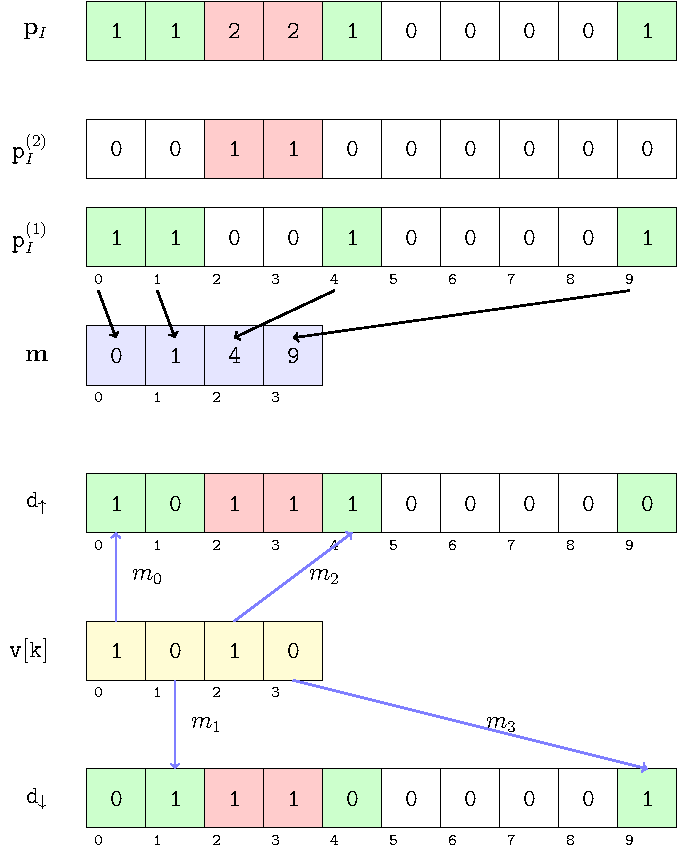
\includegraphics[width=0.9\columnwidth]{pattern.tikz} 
\caption{The {\sop} $\mpv_I$ is encoded as in Eq.~\eqref{eq:sop}. Singly and doubly
occupied orbitals are represented respectively in green and red.
The list of indices $\mathbf{m}$ of the singly occupied orbitals is built (in blue), and this
mapping is re-used to build the determinants from permutations generated by Anderson's algorithm (yellow).}
\label{fig:mapping}
\end{figure}

Figure~\ref{fig:mapping} gives a pictorial description of the data structures used to generate a determinant.
To build a generated determinant $(\md_\up,\md_\dn)$ from a permutation $\tu$, one needs to
\begin{enumerate}
    \item Fill the doubly occupied orbitals by setting both $\md_\up$ and $\md_\dn$
          equal to $\mpp_I^{(2)}$
    \item Iterate over the bits of $\tu$. If the $k$-bit is set to \one{}, set the $m_k$-th orbital of $d_\up$ to \one, otherwise set the $m_k$-th orbital of $d_\up$ to \one.
\end{enumerate}

\subsection{Further optimizations}

As a first optimization, all the possible permutations can be generated
iteratively by considering only what has changed between the previously
generated determinant and the current one.
The integer obtained by $\mathtt{v[k-1]} \oplus \mathtt{v[k]}$ has bits set at
the positions where the bits differ between $\mathtt{v[k-1]}$ and
$\mathtt{v[k]}$. The positions of these bits can be found by iteratively
\begin{enumerate}
\item counting the number of trailing zeros
\item setting the least significant {\one} to {\zero} by setting
      $\mathtt{v[k] \gets v \wedge (v-1)}$
\end{enumerate}
until $v[k] = 0$. Hence, a determinant can be generated from the previous
one in the sequence with less computational effort.

A second optimization is to consider time-reversal symmetry. When $n_\up =
n_\dn$, one can remark that $\mathtt{v[}2^{n_\up+n_\dn}-1-\mathtt{k]} = \neg \mathtt{v[k]}$.
Hence, it suffices to iterate over the half of the permutations of Anderson's
algorithm, and then generate the symmetric determinants.

%%%%%%%%%%%%%%%%%%%%%%%%%%%%%%%%%%%%%%%%%%%%%%%%%%%%%%%%%%%%%%%%%
\section{Shifted Epstein-Nesbet denominators}
%%%%%%%%%%%%%%%%%%%%%%%%%%%%%%%%%%%%%%%%%%%%%%%%%%%%%%%%%%%%%%%%%

%An advantage of \csf s over determinants is that the Epstein-Nesbet
%second-order perturbative correction is invariant with respect to the quantum
%number $m_s$. But this is not the case in the determinant basis.

Let us consider a normalized spin-pure wave function with energy $E$, expressed as
\begin{equation}
\ket{\Psi} = \sum_{i \in \mathcal{I}} c_i \ket{D_i}
\end{equation}
which is an eigenfunction of the Hamiltonian projected in the internal space of
determinants $\mathcal{I}$.
The variance of the energy associated with this function is
\begin{equation}
\sigma^2 = \mel{\Psi}{\hat{H}^2}{\Psi} - \mel{\Psi}{\hat{H}}{\Psi}^2 .
\end{equation}
Inserting the resolution of the identity for $\hat{H}^2$, 
\begin{equation}
\sigma^2 = \sum_{\alpha \in \text{FCI}} \mel{\Psi}{\hat{H}}{\alpha} \mel{\alpha}{\hat{H}}{\Psi} - E^2
\label{eq:ri}
\end{equation}
where $\text{FCI}$ denotes a complete set of are arbitrary orthonormal basis
functions, $\ket{\alpha}$, spanning the Full Configuration Interaction (FCI)
space.
The FCI space can be split in three subspaces:
\begin{itemize}
\item The internal space $\mathcal{I}$
\item The external space $\mathcal{E}$ which is the subset of $\ket{\alpha}$ which
      don't belong to $\mathcal{I}$, and for which $\mel{\Psi}{\hat{H}}{\alpha}
      \ne 0$
\item The rest of the FCI space.
\end{itemize}
$\hat{H}$ is symmetric, so Eq.~\eqref{eq:ri} can be re-written as
\begin{equation}
\sigma^2 = \sum_{D_I    \in \mathcal{I}} \mel{D_I}{\hat{H}}{\Psi}^2 
         + \sum_{\alpha \in \mathcal{E}} \mel{\Psi}{\hat{H}}{\alpha} \mel{\alpha}{\hat{H}}{\Psi} - E^2.
\end{equation}
As $\ket{\Psi}$ is an eigenfunction of $\hat{H}$ projected in $\mathcal{I}$, 
\begin{equation}
\mel{D_I}{\hat{H}}{\Psi}^2 = \left( E\, \langle D_I | \Psi \rangle \right)^2 = E^2 c_I^2,
\end{equation}
and as $\ket{\Psi}$ is normalized, one obtains
\begin{equation}
\sigma^2 = \sum_{\alpha \in \mathcal{E}} \mel{\Psi}{\hat{H}}{\alpha}\mel{\alpha}{\hat{H}}{\Psi}.
\end{equation} 

The variance of the energy is invariant with respect to the form of the
functions $\ket{\alpha}$, as long as they are orthonormal functions spanning
the space $\mathcal{E}$.  Moreover, the variance of the energy is the equal for
degenerate wave functions with different quantum numbers $m_s$.  Hence, one can
choose equivalently the $\ket{\alpha}$ to be Slater determinants or
\csf s.

The Epstein-Nesbet second-order perturbative contribution to the energy is given
by
\begin{equation}
\ept = \sum_{\alpha \in \mathcal{E}} \frac{\mel{\Psi}{\hat{H}}{\alpha}\mel{\alpha}{\hat{H}}{\Psi}}{E-\mel{\alpha}{\hat{H}}{\alpha}}.
\label{eq:pt2}
\end{equation}
This equation can be seen as a weighted sum of the different terms involved in
the expression of the variance. However, the weights differ depending on the
choice of $\ket{\alpha}$. Also, when a basis of Slater determinants is chosen,
this expression is not invariant with respect to the choice of $m_s$, which
is not desirable.

A way to cure the invariance with respect to $m_s$ is to impose all the weights
to be the same for all the determinants belonging to the same \csf . But as 
the same determinant can appear in the expression of multiple \csf s, one can
instead impose that the weight is the same for all the determinants belonging
to the same \sop .  This can be done by inserting a determinant-specific shift
to the denominator 
\begin{equation}
\ept = \sum_{\alpha \in \mathcal{E}} \frac{\mel{\Psi}{\hat{H}}{\alpha}\mel{\alpha}{\hat{H}}{\Psi}}{E-\mel{\alpha}{\hat{H}}{\alpha}+\epsilon_\alpha}.
\end{equation}
with
\begin{equation}
\epsilon_\alpha = \mel{\alpha}{\hat{H}}{\alpha} - E_\alpha
\end{equation}
where the shift is chosen to be
\begin{equation}
E_\alpha = \min_{\beta \in \text{\sop}(\alpha)} \mel{\beta}{\hat{H}}{\beta}.
\end{equation}
This choice of $E_\alpha$ is a good enough approximation to
$\mel{\alpha}{\hat{H}}{\alpha}$ in the basis of \csf s.

Although the generation of all the determinants is extremely fast, using
this approximation is quite expensive since it requires to compute
all the $\mel{\beta}{\hat{H}}{\beta}$ for each $\ket{\alpha}$.
To circumvent this problem, one can remark that for most of the contributions to
\begin{equation}
 \langle \Psi | \hat{H} | \alpha \rangle = \sum_i c_i \langle D_i | \hat{H} | \alpha \rangle
\end{equation}
$\ket{\alpha}$ is doubly excited with respect to $D_i$.
For all the determinants $D_j$ belonging to the same \sop{} as $D_i$, one can
define a double excitation operator
\begin{equation}
\hat{T}_{i\rightarrow j} D_i = D_j.
\end{equation}
Remarking that
\begin{equation}
\langle \hat{T}_{i\rightarrow j} D_i | \hat{H} | \hat{T}_{i\rightarrow j} \alpha \rangle =
\begin{cases}
\pm \langle D_i | \hat{H} | \alpha \rangle & \text{ if } \hat{T}_{i\rightarrow j} \ne 0 \\
0 & \text{otherwise},
\end{cases}
\end{equation}
all the contributions connected by $\hat{H}$ to $D_j$ will be shifted by 
\begin{align}
E_\alpha & = \langle \hat{T}_{i\rightarrow j} \alpha | \hat{H} | \hat{T}_{i\rightarrow j} \alpha \rangle - \langle \alpha | \hat{H} | \alpha \rangle \\
         & \approx \langle D_j | \hat{H} | D_j \rangle - \langle D_i | \hat{H} | D_i \rangle  = E_j
\end{align}
Hence, the shifts $E_j$ can be precomputed, and applied at no cost.




%%%%%%%%%%%%%%%%%%%%%%%%%%%%%%%%%%%%%%%%%%%%%%%%%%%%%%%%%%%%%%%%%
\section{Numerical tests}
%%%%%%%%%%%%%%%%%%%%%%%%%%%%%%%%%%%%%%%%%%%%%%%%%%%%%%%%%%%%%%%%%


%--------------------------------------------
\subsection{Open-shell system}
%--------------------------------------------

To test our implementation with a large number of open shells, we have prepared
model wave functions for the dissociated Chromium dimer in its 13-et state, separated by a
distance of $100~\AA$, using the def2-SVP basis.\cite{Weigend_2005}
At such a large distance, each Chromium atom is in its high-spin state with $6$
unpaired electrons. Two equivalent wave functions are built to initialize the sCI
calculation:
\begin{itemize}
\item The $m_s=6$ wave function, which is a single determinant with $30$ $\up$
      and $18$ $\dn$ electrons.
\item The $m_s=0$ 13-et wave function with $24$ $\up$ and $24$ $\dn$ electrons, which
      contains 924 determinants
\end{itemize}
The system is composed of $62$ molecular orbitals, so for this simple case $\Nint=1$.
The orbitals were obtained at the restricted open-shell Hartree-Fock (ROHF) level
for $m_s=6$.
The selection is performed in the valence Full-CI space, with $20$ frozen electrons.


%E(ROHF,ms=6) = -2086.393627426404
%E(ROHF,ms=0) = -2086.393627426463

The $m_s=0$ wave function was initialized by taking the {\sop} of the single determinant
of the $m_s=6$ wave function, and generating all the possible determinants using 
the algorithm presented in the previous section.
The generation of the $924$ determinants was done in $\sim 19~200$ CPU cycles,
i.e. $21$~cycles per generated determinant. The Hamiltonian was diagonalized and
we checked that the lowest state with $\langle \stwo \rangle = 42$ had the exact
same energy as the $m_s=6$ single determinant.


%--------------------------------------------
\subsection{Closed-shell system}
%--------------------------------------------


%%%%%%%%%%%%%%%%%%%%%%%%%%%%%%%%%%%%%%%%%%%%%%%%%%%%%%%%%%%%%%%%%
\section{Conclusion}
%%%%%%%%%%%%%%%%%%%%%%%%%%%%%%%%%%%%%%%%%%%%%%%%%%%%%%%%%%%%%%%%%

We have presented a general algorithm to complement an arbitrary wave function
with all the required determinants to obtain eigenstates of the $\stwo$
operator when the Hamiltonian is diagonalized, in a negligible time.

%%%%%%%%%%%%%%%%%%%%%%%%%%%%%%%%%%%%%%%%%%%%%%%%%%%%%%%%%%%%%%%%%

\begin{acknowledgments}
The authors gratefully acknowledge Sean Eron Anderson for creating the 
\emph{Bit Twiddling Hacks} web page.
This work was performed using HPC resources from CALMIP (Toulouse) under
allocations 2018-0510 and 2018-18005 and from GENCI-TGCC (Grant
2018-A0040801738).
\end{acknowledgments}

%%%%%%%%%%%%%%%%%%%%%%%%%%%%%%%%%%%%%%%%%%%%%%%%%%%%%%%%%%%%%%%%%

\bibliography{s2}

\end{document}
